\chapter{modified Quadratic Estimator}
\label{ch:analysis}
\section*{Overview}\label{ovr}
In this chapter we discuss modified Quadratic Estimator which we developed to eliminate the bias due thermal Sunyaev Zel'dovich (SZ) effect. 
We give a breif review thermal Sunayev-Zel'dovich effect (refer \pending{citations} for a detailed review)and its effect on cluster lensing in the \S\ref{tsz}.
Then we discuss the modifications of the QE to remove SZ bias in \S\ref{sec_method}.
 Later we explain the SPTpol and DES data sets in \S\ref{sec_data} and results in \S\ref{sec_results}
Finally we conclude in \S\ref{sec_conclusions}.
%We explain the constraints on mass-richness scaling relation obtained using the above data. 


\section{Thermal Sunayev-Zel'dovich effect}\label{tsz}

 Cosmic microwave background (CMB) photons gets inverse thompson scattered off the high energetic electrons present in the intra cluster medium of a galaxy cluster, resulting in a deficiency of photons at lower frequency and excess of photons at higher frequency. 
 This phenomena is called thermal Sunayev-Zel'dovich effect (SZ). 
 SZ is a small effect and to illustrate it we have shown CMB spectral distortion for a fictional galaxy cluster of mass 1000 times more that of a typical galaxy cluster in Figure \pending{i}.
 As shown in the fig, SZ decreases the intensity of CMB below frequency of 218 \,GHz and increase at higher frequencies. 
   
The SZ spectral distortion of the CMB expressed as a temperature change $\Delta T_{SZ}$ is given by 
\begin{equation}
\frac{\Delta T_{SZ}}{T_{CMB}} = f(x) y = f(x) \int n_{e} \frac{k_{B}T_{e}}{m_{e}c^{2}} \sigma_{T} dl
\end{equation}
where y is compton parameter, $n_{e}$ is the electron number density, $m_{e}$ is the electron rest mass, $c$ is the speed of light,  $T_{e}$ is the electron temperature, $\sigma_{T}$ is the Thompson cross-section f(x) is the dimensional frequency given by 
 The compton y parameter of SZ effect is given by 
 \begin{equation}
 x = y
 \end{equation}
 
 
 SZ effect is an order of magnitude greater than the lensing signal and hence induces a significant systematic and statistical uncertainty if not taken into account. 
 Fig ~\ref{sZ_effect} shows the effect of tSZ on the lensing convergence profile. 
 In the left panel of figure we show the stacked lensing convergence profile of 1000 clusters each with a mass of $4*10^{14}$ $M_{\odot}$ and an experimental noise of 1\ukam with no tSZ and on the right panel is with the tSZ.  
 As can be inferred from the plot, presence of tSZ induces a blue blob in the center and hence resulting in a negative bias.
 \pending{more about tSZ??`}
 \begin{figure}
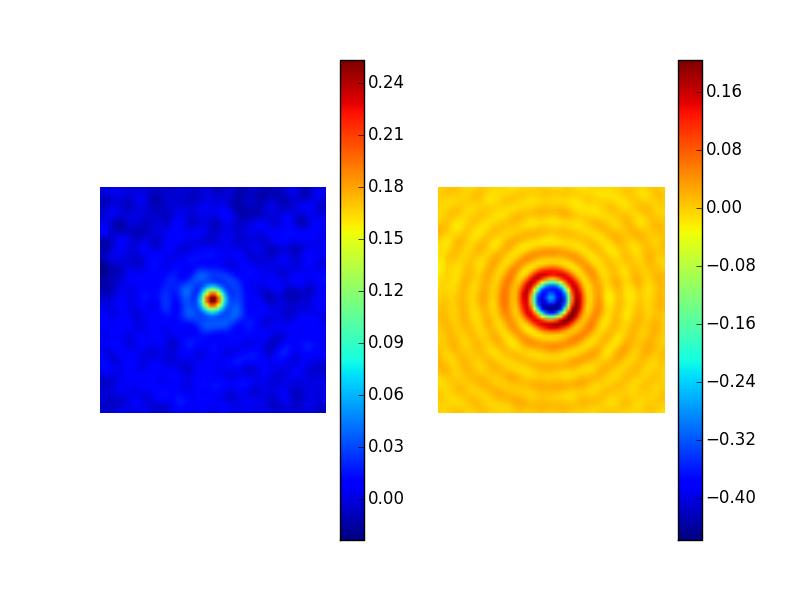
\includegraphics[width=\linewidth]{figs/tSZ_effect_on_lensing.png}
\caption{Effect of tSZ on lensing convergence profile. }
\label{fig:SZ_effect}
\end{figure}



%In this section we briefly introduce the \sptpol{} and DES surveys.
%Next we describe \planck{} data products and the selection of the cluster catalog for the lensing analysis.
\section{Data}
\label{sec_data}
\pending{More on SPT survey}
We use data sets from two different experiments: CMB maps from South Pole Telescope are explained in \S\ref{sec_SPT} and 
optical cluster catalog from Dark Energy Survey which is explained in \S\ref{sec_DES}

\section{South Pole Telescope}
\label{sec_SPT}
South Pole Telescope (SPT) is a 10 meter diameter, wide field, offset Gregorian telescope \citep[SPT,][]{padin08, carlstrom11} located at the Amundsen-Scott South Pole station.
The SPT has been operating since early 2007 and has completed two surveys so far: SPT-SZ (2007 -2011) and SPTpol (2012-2016).  
Extremely dry and stable atmosphere of the south pole makes it one of the best available sites on Earth for observing millimeter and sub-millimeter wavelengths. 

\subsection{\sptpol{} {\rm 500} deg$^{2}$ survey}\label{sec_sptpol}
\sptpol{} is the second camera installed on the \mbox{10-meter} South Pole Telescope \citep[SPT,][]{padin08, carlstrom11} located at the Amundsen-Scott South Pole station.
The \sptpol{} focal plane consists of 1536 polarization-sensitive transition edge sensor bolometers (360 at 95 GHz and 1176 at 150 GHz) \citep{austermann12}.
%enabling polarization observations \citep{austermann12}.
The \sptpol{} 500~deg$^{2}$ survey spans fifteen degrees of declination, from -65 to -50 degrees, and four hours of right ascension, from 22h to 2h. 
%In this work we use the temperature (T) and polarization (Stokes Q and U) maps of the CMB from observations between April 2013 to September 2016 in the frequency bands 95 GHz and 150 GHz. 
In this work, we use CMB temperature maps from observations between April 2013 and September 2016 in frequency bands centered at approximately 95 GHz and 150 GHz. 
The telescope beam and pointing solutions were characterized using Venus and bright point sources in the \sptpol{} survey region. 
The final telescope beam along with the pointing jitter roughly corresponds to a $\theta_{\rm FWHM} = 1.^{\prime}22\ (1.^{\prime}7)$ Gaussian for the 150 (95) GHz dataset.

We briefly summarize the procedure we use to reduce raw CMB data to maps and refer the reader to \cite{henning18} for further details. 
The raw data are composed of digitized time-ordered data (TOD) for each detector that are converted into CMB temperature units. %% using a Planck-based calibration factor. 
We bin the TOD into two different maps using a flat-sky approximation in the Sanson-Flamsteed projection \citep{calabretta02, schaffer11}. 
To construct the first map, in which we aim to reconstruct the small-scale lensing signal, we remove large-scale modes $\ell \le 300$, bandpass filter the TOD in the range of approximately $300 \le \ell_{x} \le 20,000$, and bin them into 0.\am5\ square pixels.
For the second map, intended for estimation of the large-scale CMB gradient, we apply minimal TOD filtering by only removing modes below $\ell_{x} \le 30$, and bin them into 3\am\ square pixels.
While we only use the data from the 150 GHz channel for the first map, the latter is a tSZ signal cleaned map produced by linearly combining the 95 and 150 GHz channels. 
We use this tSZ-free map to reconstruct the background gradient of the CMB at the cluster locations.
As we will see later in \S\ref{sec_method_QE}, the gradient estimation using the tSZ-free map helps in removing the tSZ-induced lensing bias.
The minimal filtering on this map allows us to recover large-scale modes which indeed helps in a better estimation of the background gradient.
The 0.\am5{} resolution 150 GHz map has a white noise level of \mbox{$\Delta_{\rm T} = $ 6 \ukam} estimated using a jackknife approach. %estimated within the multipole band $4500 \le \ell \le 7500$.
The low-resolution tSZ-free combination is noisier with \mbox{$\Delta_{\rm T} \sim $ 17 \ukam}.
%%%\pending{Pending: SR: Should we quote this? Can we trust this number?}
%\section*{Cosmic Microwave Background cluster lensing}
\subsection{DES and the {\rm \RM} catalog}\label{sec_DES}
The Dark Energy Survey (DES) is a $\sim$5000 \sqdeg, optical to near-infrared survey conducted using the Dark Energy Camera \citep{flaugher15} mounted on the 4-meter Victor Blanco telescope at Cerro Tololo Observatory in Chile and has recently begun its sixth year of observations. 
For this analysis, we use the cluster catalog obtained from the first three years of DES observations, which almost covers the \sptpol{} 500\,deg$^{2}$ survey. 

%The cluster catalog was derived using the RM algorithm \citep{rykoff14}  from the DES photometric datasets. 
The cluster catalog was derived using the RM algorithm \citep{rykoff14}.
RM is an optical cluster-finding algorithm which detects candidates by identifying over-densities of luminous red galaxies with luminosity greater than 20\% of $L_{*}.$
%Milky Way ($0.2L_{*}$). [I DON'T THINK THIS IS ACTUALLY THE DEFINITION OF L* (TC\citetalias{mcclintock18})]
It is based on our understanding that galaxy clusters are agglomerations of galaxies containing old and subsequently red stars. 
The algorithm iteratively assigns membership and centering probabilities for each red galaxy identified as belonging to a cluster candidate. 
A weighted sum of the membership probabilities, richness $\lambda$, is assigned to each candidate.
The centre comes from the galaxy with the highest centering probability.
The DES RM catalog contains two samples: a flux-limited sample and a volume-limited sample. 
The flux-limited sample has more high-redshift clusters detected from deep fields in the survey. 
On the other hand, the volume-limited sample is independent of survey depth, complete above a luminosity threshold \citep[hereafter \citetalias{mcclintock18}]{mcclintock18}, and normally preferred for cosmological analysis.
% (hereafter referred to as the volume-limited sample).
See \citet{rykoff16} for more information on the application of RM to the DES survey data.

The RM cluster catalog version employed in this analysis is \whichcatversion. 
The \whichyear{} gold catalogue is based on the previous catalog from the Year-1 data \citep{drlica-wagner17} with some updates described in \citet{morganson18}.
The catalog contains 54,112 clusters above richness $\lambda \ge 20$ in the flux-limited sample and 21,094 clusters in the volume-limited sample. % \pending{(Pending: Cite DES Y3 cat. paper)}. 
Of these, 5,828 (2,428) clusters from the flux(volume)-limited sample lie within the \sptpol{} 500 \sqdeg{} survey  in the redshift range $0.1 \le z \le$ 0.95 (0.90). 
%We additionally remove clusters near the survey edges or within $10^{\prime}$ distance from a bright ($\ge 50$ mJy at 150\,GHz) point source.
We additionally remove clusters near the survey edges by removing the cutouts (see \ref{sec_cluster_cutouts}) with more than 5\% masked pixels or within $10^{\prime}$ distance from any bright ($\ge 6$ mJy at 150\,GHz) point sources detected in the \sptpol{} temperature map.
%we use data/500sqdeg_bleem/quick_mm_point_source_file_150.0GHz_6.00000mJy.txt.
These cuts leave 4,003 (1,741) clusters with $\lambda \ge 20$ from the flux(volume)-limited sample with a median redshift of $\tilde{z}$ = 0.77 (0.48). 
The error in the cluster photo-$z$ estimates are small with $\hat{\sigma}_{z} = 0.01 (1+z)$ \citep{rozo15}.
\pending{include a figure with SPTpol map and pointing to a cluster}
%\pending{Finally, we impose a cut on the cluster richness and remove all clusters above $\lambda \ge 60$ that removes \pending{xx (xx)} from the full (cosmology) sample. This cut was motivated based on the results from Sehgal sims described in \S\ref{sec_xx_xx}}.
%Cosmic Microwave Background (CMB) photons while passiang through intervening galaxy cluster gets lensed and we call this phenomenon as CMB-cluster lensing.
% Lensing remaps the unlensed CMB field based on the angular deflection caused by cluster gravitational potential.
 %In mathematical form CMB cluster lensing can be written as the equation below
 %\begin{eqnarray}
%T(\hat{\textbf{n}})& = & \widetilde{T} (\hat{\textbf{n}} + \vec{\alpha}(\hat{\textbf{n}}))\\
%Q(\hat{\textbf{n}}) & = & \widetilde{Q} (\hat{\textbf{n}} + \vec{\alpha}(\hat{\textbf{n}}))\\
%U(\hat{\textbf{n}}) & = & \widetilde{U} (\hat{\textbf{n}} + \vec{\alpha}(\hat{\textbf{n}}))
%\end{eqnarray}
%where $ \widetilde{T}$ is unlensed temperature field, $\widetilde{U}$ and $\widetilde{Q}$ are the unlensed polarisation fields.
%$\vec{\alpha}(\hat{\textbf{n}})$ denotes the deflection angle and is directly proportional to the mass of the galaxy cluster.

%Lensing signal by an individual cluster is too weak to detect, so we need to stack many clusters to obtain a significant signal.
 %For example, the lensing induced distortion due to a $2 \times 10^{14} \ M_{\odot}$ mass galaxy cluster  is $\sim 5.0$ and $0.5 \ \mu K$ in temperature and polarization respectively.
%In this chapter, we will discuss various methods available in literature to extract CMB-cluster lensing signal. 
%The chapter is organized as follows 
\section{Methods}
\label{sec_method}
\section{Quadratic Estimator}
%Quadratic Estimator is based on two approximations: gradient approximation and linearization in convergence.

Typical size of galaxy cluster is of the order of few arc minutes. 
Primordial CMB doesn't have power at such small scales due to diffusion damping \cite{Silk} and can be approximated as a gradient. 
Lensing due to galaxy cluster induces a dipole kind of structure oriented along the direction of background gradient with hot and cold spots swapped.
For a given cluster mass and redshift, the magnitude of this dipole scales linearly with the magnitude of the CMB gradient.
This correlation between the unlensed CMB gradient and lensing signal is known as the gradient approximation and is equivalent to
\begin{equation}
T (\hat{n})\approx \tilde{T}+ \nabla T . \vec{\alpha}(\hat{\textbf{n}})
\end{equation}
Below we provide the mathematical formalism for temperature quadratic estimator and it generalises for polarisation.

 Under the gradient approximation, we construct an estimator of lensing convergence by multiplying the lensing map and the gradient map.
The gradient approximation doesn't hold for all Fourier modes, only for the modes which are correlated by reconstruction.
Hence we filter maps in the Fourier space to isolate modes for which the gradient approximation is valid.
%\begin{equation}
% \hat{k_{l}} = -A_{l} \int d^{2} \hat{n} e^{i\hat{n}.l} Re{\nabla .[G(\hat{n}) L^{*}(\hat{n})]}
 %\end{equation}
 We obtain gradient and lensing maps as follows,
 % $G(\hat{n})$, $L(\hat{n})$ are filtered gradient and lensing maps respectively, $A_{l}$ is the normalisation parameter.
 % We obtain $G(\hat{n})$, $L(\hat{n})$ from the observed temperature map as follows
  \begin{eqnarray}
  L(\hat{n}) = \int \frac{d^{2}l}{(2\pi)^{2}} e^{il .\hat{n}} W^{T}_{l} T_{l}\\
  G(\hat{n}) = \nabla (\int\frac{d^{2}l}{(2\pi)^{2}} e^{il .\hat{n}} W^{TT}_{l} T_{l}   )
  \end{eqnarray}
  where $G(\hat{n})$, $L(\hat{n})$ are filtered gradient and lensing maps and $T_{l}$ is the observed temperature map in fourier space.  
 Fourier filters $W^{T}_{l}$ and $W^{TT}_{l}$ are given by 
 \begin{eqnarray}
 W^{T}_{l} = (C^{TT}_{l} + N^{TT}_{l})^{-1}\\
 W^{TT}_{l} =  \widetilde{C}^{TT}_{l}(C^{TT}_{l} + N^{TT}_{l})^{-1}
 \end{eqnarray}
 where  $\widetilde{C}^{TT}_{l}$,$C^{TT}_{l} $  is the unlensed and large scale structure lensed CMB power spectrum, $ N^{TT}_{l}$ is the noise power spectrum.
 With filtered gradient and lensing maps in hand we can write down the expression for lensing convergence profile as 
 \begin{equation}
 \hat{k_{l}} = -A_{l} \int d^{2} \hat{n} e^{i\hat{n}.l} Re{\nabla .[G(\hat{n}) L^{*}(\hat{n})]}
 \end{equation}
 where $A_{l}$ is the normalisation parameter given by
 \begin{equation}
 \frac{1}{A_{l}} = \frac{2}{l^{2}} \int \frac{d^{2}l_{1}}{4\pi^{2}} (l.l_{1}) W^{TT}_{l} W^{T}_{l} (\tilde{C}^{TT}_{l_{1}}(l.l_{1}) + \tilde{C}^{TT}_{l_{2}}(l.l_{2}))
 \end{equation}
 where $l = l_{1}  + l_{2}$. 
  \subsection{mitigating magnification bias}
Galaxy cluster magnifies the background image and decreases the observed temperature gradient behind it , which leads to a low bias in reconstruction.
The bias is due to the overlap in scales between the unlensed temperature gradient and the lensed temperature field. 
Though wiener filter reduces the bias, it is not removed completely.
We can reduce the bias further by exploiting the prior knowledge on unlensed CMB power spectrum.
 From Fig.~\ref{fig:gradient_cut} which shows the unlensed rms gradient as a function of multipoles, it is evident that most of the power for the gradient map comes from scales below l<2000.
 So by low pass filtering the gradient map, we separate the unlensed temperature gradient and the lensed temperature field with almost no loss in SNR.
 \begin{figure}
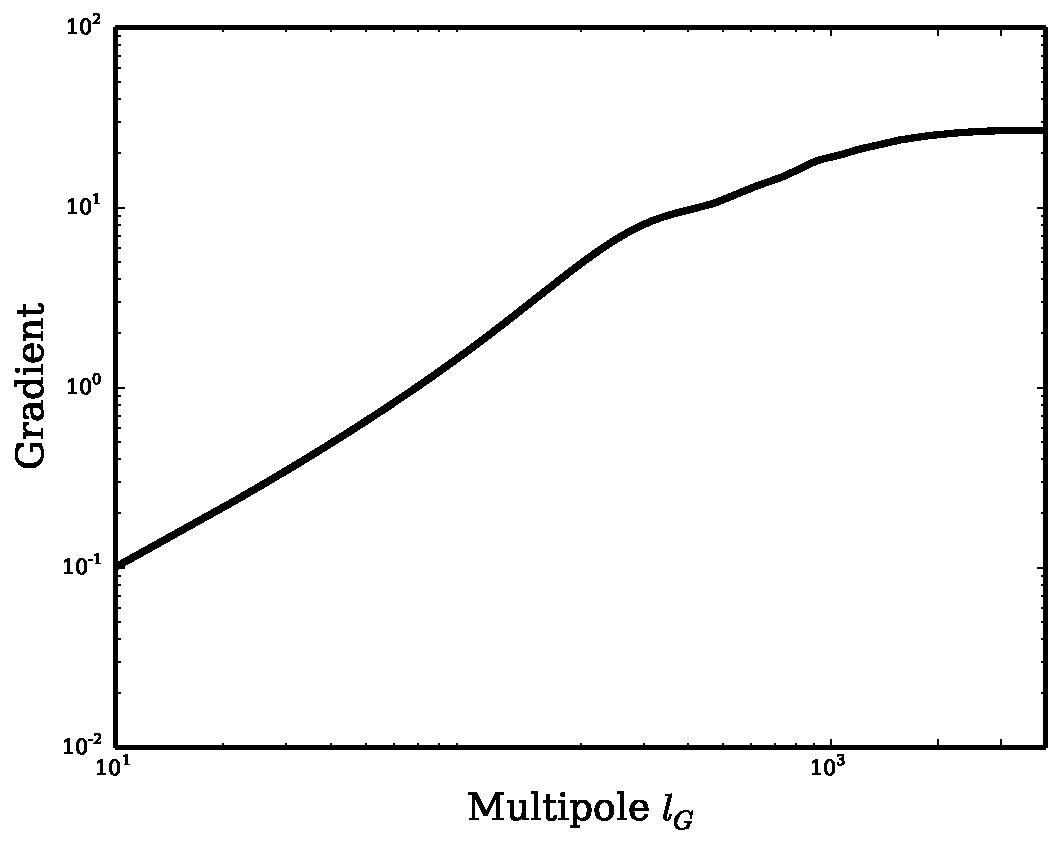
\includegraphics[width=\linewidth]{figs/gradient_cut.pdf}
\caption{Gradient of temperature field as a function of low pass filter l = $l_{G}$. It is dominated by mulitpoles below 2000. \pending{check the magnitude of Grms}}
\label{fig:gradient_cut}
\end{figure}
 \subsection{fitting model}
To obtain the mass of the cluster, we need compare the observed lensing profile to the convergence model generated using an assumed halo mass profile.
 For that we assume the galaxy cluster density to follow Navarro Frenk White (NFW) profile.
 A NFW halo profile is characterized by its scale radius $R_{s}$, the dimensionless concentration parameter c, and the dimensionless charateristic over-density $\delta_{c}$.
 The characteristic over density is defined as the ratio central cluster density to the critical density of the Universe at the cluster redshift.
 In terms of these quantities the NFW halo density profile is written as 
 \begin{equation}
 \rho(r) = \frac{\delta_{c}\rho_{crit,z}}{(\frac{r}{R_{s}})(1 + \frac{r}{R_{s}})^{2}}
 \end{equation} 
 where $\rho_{crit,z}$ is the critical density of the Universe at cluster redshfit.
 
 The lensing convergence profile is the ratio of surface mass density to the critical surface density of the Universe at cluster redshift, $k(x) = \frac{\Sigma(x)}{\Sigma_{crit}}$, where
 \begin{eqnarray}
 \Sigma(x) = 2 \int^{\inf}_{0} \rho(r) ds\\
 \Sigma(crit) = \frac{c^{2}}{4\pi G} \frac{D_{CMB}}{D_{clus} D_{CMB,clus}} 
 \end{eqnarray} 
Here r is the distance from the center, x is the corresponding projection on the plane, is the distance along the line of sight, $D_{CMB}$, $D_{clus}$ are the comoving distances to the CMB and galaxy cluster respectively and $D_{CMB,clus}$ is the distance between the CMB and the cluster.


With model prediction in hand we can write down the likelihood of observing the data as:
\begin{equation}
-2 ln L (k | M) = (k - k_{m})(M) C^{-1} [(k - k_{m})]^{T}
\end{equation}
where k is the observed lensing convergence profile, $k_{m}$ is lensing convergence for NFW profile at mass M, C is the covariance matrix. 

%\section{NFW profile}
The schematic representation of Quadratic Estimator is shown in Fig 2. 
Panel (a) is the 10' X 10' cutout of the observed temperature map, $T_{l}$.
This is filtered in the fourier space \pending{mention equations} to obtain the filtered gradient and lensing maps, shown in panel (b) and (c) respectively.
Lensing convergence profile (panel (c)) is reconstructed by extracting the correlations between lensing and gradient maps.
 \begin{figure}[H]
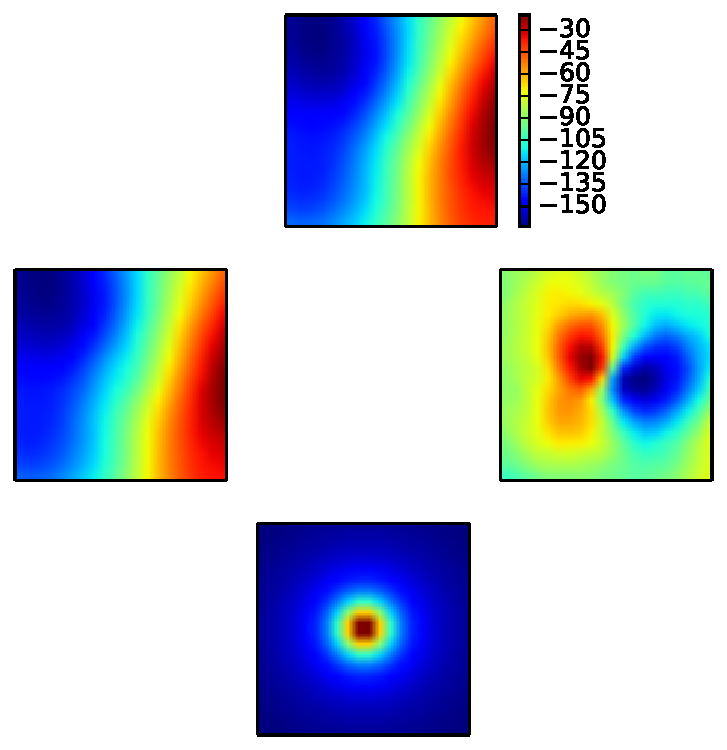
\includegraphics[width=\linewidth]{figs/schematic_rep.pdf}
\caption{Gradient of temperature field as a function of low pass filter l = $l_{G}$. It is dominated by mulitpoles below 2000. \pending{check the magnitude of Grms}}
\label{fig:gradient_cut}
\end{figure}
 
\section{modifications of Quadratic Estimator}
The major foreground in CMB cluster lensing analysis is thermal Sunyaey -Zel'dovich (tSZ) effect. 
tSZ effect is an order of magnitude greater than lensing signal; if not taken into consideration it induces systematic bias and varianace in the final convergence maps.
In this section we describe the modifications of Quadratic Estimator to make it robust to both tSZ induced bias and variance.

\subsection{modified Quadratic Estimator}
While designed to pull the lensing induced correlations, QE is equally sensitive to any other signal present in both G and L maps.
%The major systematic for lensing analysis is thermal Sunyaey -Zel'dovich (tSZ) effect, which is an order of magnitude greater than lensing signal biases the analysis if not taken into account. 
 tSZ present in both maps results in a low bias.
 One way to eliminate tSZ bias is using tSZ free maps, which are constructed by exploiting the frequency dependance of tSZ signal.
 %Previous studies either used a tSZ free map or a more stringent low pass filtering of the gradient map.
 %tSZ is frequency dependent signal and hence we can use multiple frequency channels to eliminate tSZ. 
 However, this results in a increased statistical uncertainty in the reconstructed convergence profile.
 Another way to mitigate the bias is by using a more stringent low pass filter on the gradient map. %; by having a more robust seperation of scales between gradient map and small scale map.
 By having a more robust seperation of scales between gradient map and small scale map.
 While this can reduce the bias significantly, this results in a poor gradient estimation and hence increasing the statistically uncertainty.

 
 During my thesis we came up with a novel approach to completely remove the tSZ bias. 
 Any foreground signal which is present in both the maps will lead to a systematic bias, so by getting rid of the foreground signal in one of the maps (either G or L) should eliminate the bias completely.
  As shown in Fig.~\ref{fig:gradient_cut}, most of the gradient estimation comes from multipoles l <2000 and CMB is not limited by noise at those scales.
  So, natural choice would be to eliminate tSZ in the gradient map by using linear combination of different frequencies. 
  In modified Quadratic Estimator, eqn 3.6 becomes,
  \begin{equation}
   G(\hat{n}) = \nabla (\int\frac{d^{2}l}{(2\pi)^{2}} e^{il .\hat{n}} W^{TT}_{l} T^{SZ_free}_{l}   )
  \end{equation}
  where $T^{SZ_free}_{l} $ is the tSZ-free map.
  \section{Results and Discussion}\label{sec_results}

The main results of this work are the lensing-derived cluster mass constraints for the DES RM \whichyear\ cluster samples using \sptpol{} tSZ-free $\times$ 150 GHz temperature maps.
%using three different combination of the \sptpol{} and \planck{} temperature maps: (A) \sptpol{} tSZ-free $\times$ 150 GHz maps (baseline); (B) \lgmca $\times$ \sptpol 150 GHz maps; and (C) baseline $+$ \sptpol{} tSZ-free $\times$ tSZ-free maps for clusters with $\lambda \ga 40$.
Below, we first present the lensing mass estimates in \S\ref{sec_temp_results} and use the lensing measurements from the DES \whichyear{} volume-limited sample to independently calibrate the \ML{} relation of the cluster sample in %\S\ref{sec_ML_scaling}. 
\subsection{Stacked mass measurements}
\label{sec_temp_results}
In Fig. \ref{fig_QE_stacked_maps}, we present the results of our stacked lensing measurements. 
The left (right) panel correspond to the convergence maps stacked at the location of clusters in the DES \whichyear\ flux(volume)-limited sample.
The variance in the flux-limited sample is lower than the volume-limited sample because the flux-limited sample has twice as many objects. 
An estimate of the mean-field has been subtracted from the maps.
We reject the null hypothesis of no lensing with a significance of \howmanysigmaforfullsample\ for the flux-limited sample of \howmanyclustersinfullsample\ clusters. 
The obtained \snr{} is consistent with our expectations from the simulations shown as lighter black circles in %Fig. \ref{fig_QE_sehgal_sims}.
For the smaller volume-limited sample, the no-lensing hypothesis is ruled out at  \howmanysigmaforcosmosample.
The radially binned convergence profiles that are used to estimate the cluster masses are shown in Fig. \ref{fig_QE_stacked_maps_radprf} along with the best-fit model curves. 
\begin{figure}
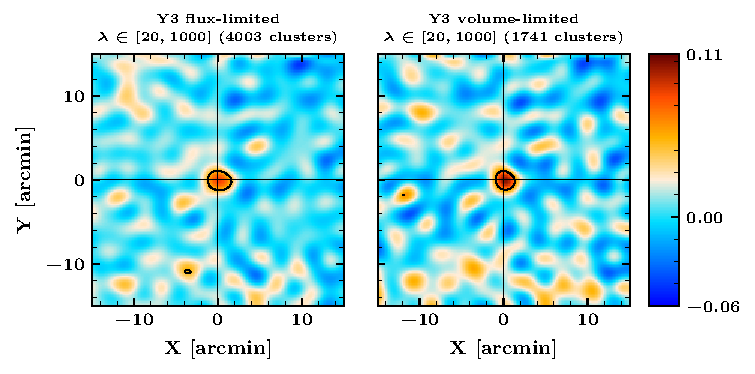
\includegraphics[width=\linewidth]{figs/kappa_model_MF_y3_v6_4_22_full_vl_JODY.pdf}
\caption{It shows}
\label{fig:fig_QE_stacked_maps}
\end{figure}

\begin{figure}
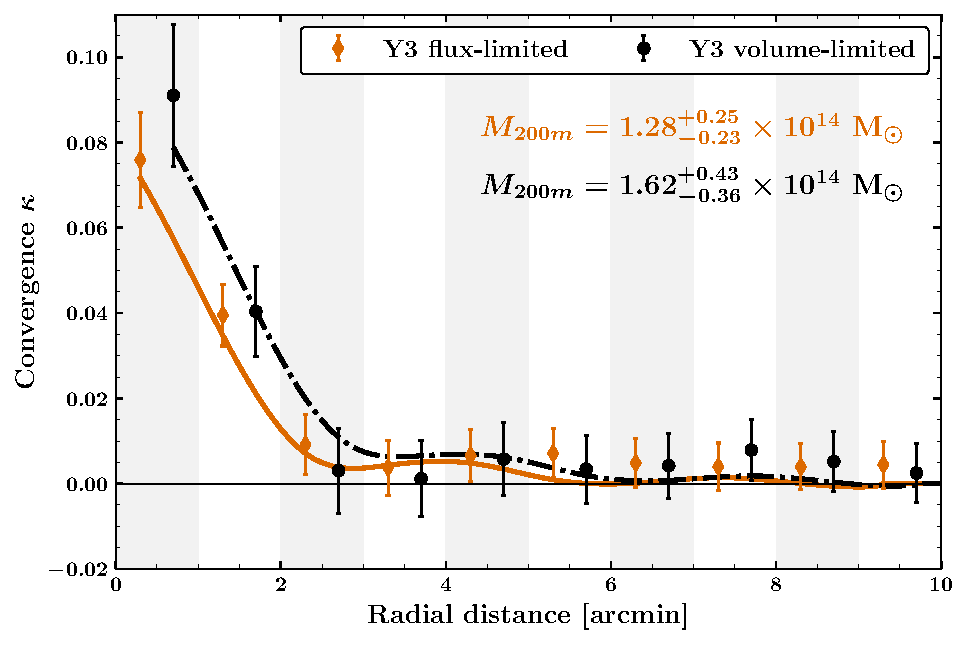
\includegraphics[width=\linewidth]{figs/kappa_model_MF_y3_v6_4_22_full_vl_radprf_JODY.pdf}
\caption{It shows}
\label{fig:fig_QE_stacked_maps}
\end{figure}

The ringing pattern is because of the sharp filtering of modes above the \sptpol{} beam scale. 
The error bars plotted are the square root of the diagonal entries of the covariance matrix estimated using %Eq. (\ref{eq_JK_cov}). 
%As explained in \S\ref{sec_nfw_model_fitting}, all the mass estimates are derived by fitting a NFW profile along with the contribution from the {\it 2-halo} term to the measured radially binned profile. 
The recovered lensing masses for the stacked flux and volume-limited samples are %\mbox{\mvir = \fitmassforfullsamplewitherrors\ \times \munits} and \mbox{\fitmassforvlsamplewitherrors\ \times \munits} respectively. 
According to expectations, the lensing masses shift up by 0.3$\sigma$ when the {\it 2-halo} term is excluded.


A higher mean mass is expected for the volume-limited sample. 
At redshifts above $z\sim 0.6$, galaxies at the luminosity threshold adopted by RM become too faint to be detected in the DES data. 
Consequently, the richness of the clusters is extrapolated from the subset of galaxies that are sufficiently bright to be detected. 
This extrapolation introduces additional noise in the richness estimates.
The increased scatter leads to more low-mass systems scattering up to apparently rich systems, thereby lowering the mean mass of the selected halos. 
For this reason, we restrict our analysis to the volume-limited sample in the subsequent sections. 
\subsection{Mass-richness \ML{} scaling relation calibration}\label{sec_ML_scaling}

We now apply the lensing mass measurements from \S\ref{sec_temp_results} to constrain the relationship between a cluster's mass, $M$, and optical richness, $\lambda$, in the DES RM \whichyear{} volume-limited sample. 
We limit the analysis to just the volume-limited sample since the flux-limited sample has selection bias as explained above in \S\ref{sec_temp_results}.
%Due to its higher S/N, we use the QE  with a tSZ-free gradient map; we do not combine the two estimators due to the complexity in combining the different bases of the MLE and QE. 
Following earlier weak-lensing analyses of RM clusters \citep{simet18, melchoir17, mcclintock18}, we use a power-law scaling relation for cluster mass, $M$, as a function of richness, $\lambda$, and redshift, $z$,
\begin{eqnarray}
M = A \left(\frac{\lambda}{40}\right)^{\alpha} \left(\frac{1+z}{1+0.35}\right)^{\beta},
\label{eq_ML}
 \end{eqnarray}
 where $A$ is a normalization parameter, and the exponents $\alpha$ and $\beta$ are richness and redshift evolution parameters respectively. 
The pivot points for the richness and redshift evolution were set based on DES weak-lensing measurements of \citetalias{mcclintock18}.
%Given the total\snr{}is of order eight for the flux-limited sample, we do not subdivide the stacks into different richness or redshift bins. 
The model for the stacked mass is 
\begin{equation}
M(A, \alpha, \beta) \equiv M = \frac{\sum_j w_j M(\lambda_{j}, z_{j})}{\sum_j w_j}, 
\label{eq_model_ML}
\end{equation}
where the sum runs over the number of clusters in the sample and the weight $w$ for each cluster is given in Eq. (\ref{eq_cluster_weight}).

We do not split the stacks into different richness or redshift bins.
As a result, the data's sensitivity to the two evolution parameters is minimal and we apply informative priors to both.
We perform a Markov chain Monte Carlo (MCMC) analysis %with 100 walkers and 750 steps each 
using the publicly available \emph{emcee} \citep{mackey13} code to sample the likelihood space.
%The first 100 steps from all walkers were discarded as the burn-in phase.
\begin{figure}
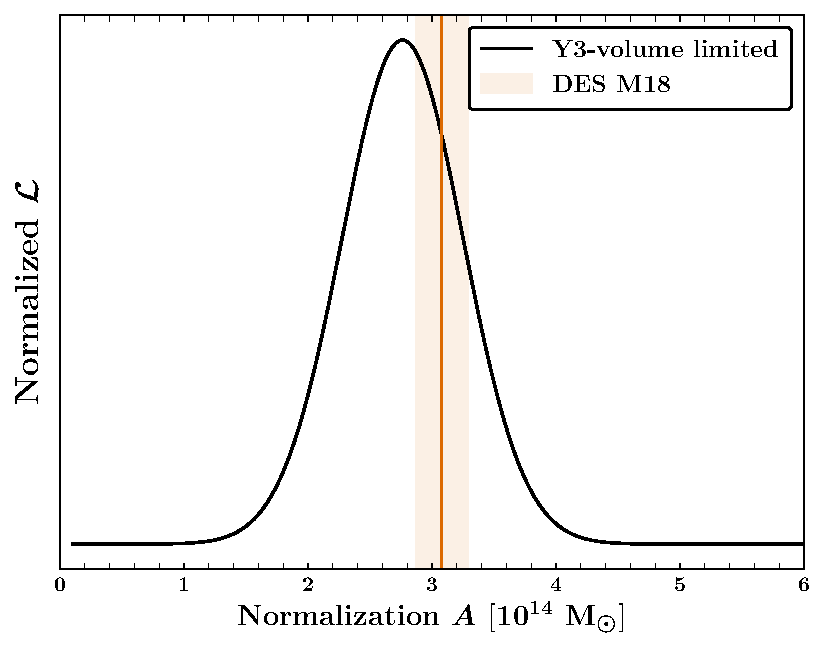
\includegraphics[width=\linewidth]{figs/M_rich_fitting_y3_v6_4_22_full_vl_JODY.pdf}
\caption{It shows}
\end{figure}